\chapter{Introducción y Objetivos}
\section{Objetivos del curso.}
El objetivo global del curso es la introducción de los elementos básicos para llevar a cabo el cálculo y diseño de una estructura:
\begin{itemize}
    \item Tipologías estructurales.
    \item Materiales.
    \item Prestaciones exigidas
    \item Acciones
    \item Cálculo estructural
\end{itemize}

\section{Tipos de esfuerzo. Cálculo elástico/plástico.}
\begin{figure}[h]
    \centering
    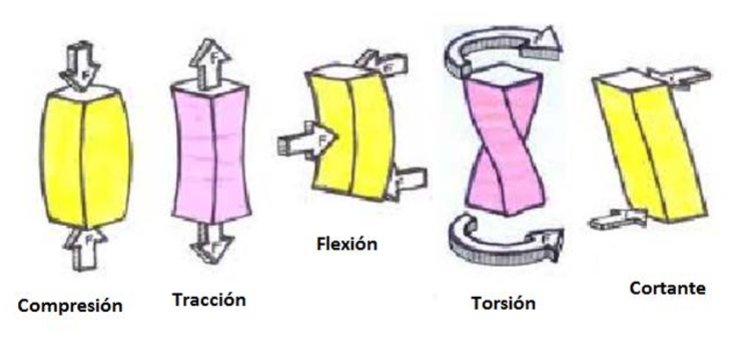
\includegraphics[width=0.75\linewidth]{Imagenes/Tipos de esfuerzo.png}
    \caption{Tipos de esfuerzo.}
\end{figure}

\begin{figure}[h]
    \centering
    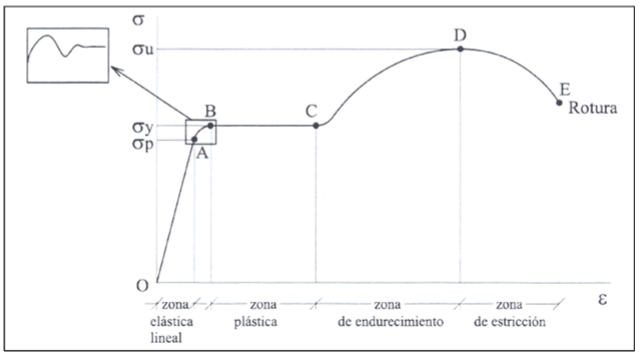
\includegraphics[width=0.75\linewidth]{Imagenes/Diagrama deformacion.png}
    \caption{Curva de esfuerzo-deformación.}
\end{figure}

\subsection{Cálculo Elástico.}
Los elementos estructurales deben de permanecer en el rango elástico. Esfuerzos y deformaciones en régimen lineal.

\subsection{Cálculo Plástico (Diseño a la rotura).}
Se permite que los elementos estructurales entren en el rango plástico. Se determinan las cargas y mecanismos de colapso

A la hora de diseñar el mismo elemento con ambas teorías, con el diseño a la rotura se obtienen dimensiones y cuantía del material menores que al hacerlo con un diseño elástico, ya que se necesitará mayor dimensión y cuantía del material para mantener el material en el rango elástico ante un mismo esfuerzo.

\section{Proyecto estructural.}
\subsection{Procedimiento.}
\begin{figure}[h]
    \centering
    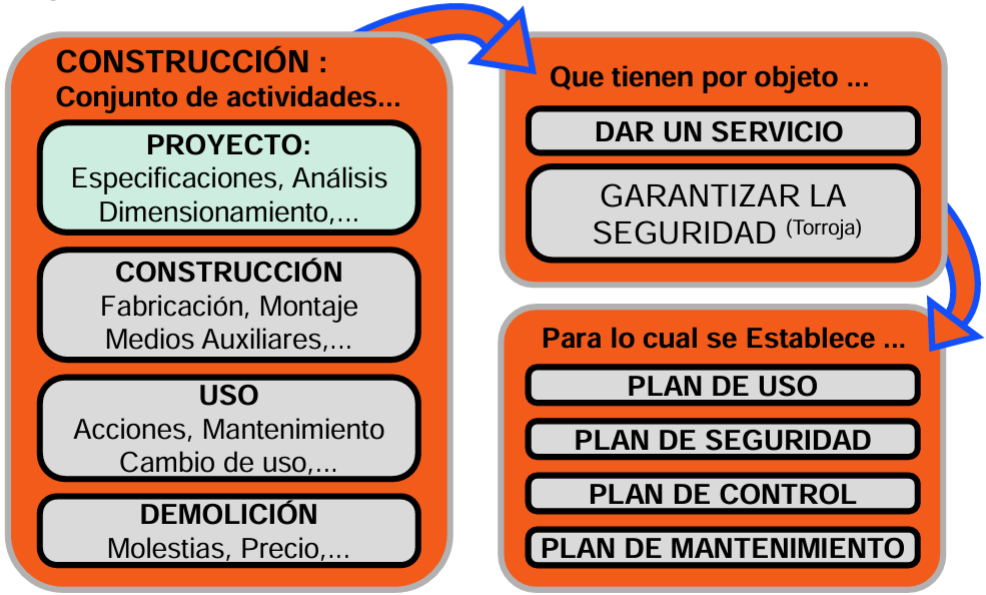
\includegraphics[width=0.75\linewidth]{Imagenes/Proyecto estructural. Procedimiento.png}
\end{figure}

Procedimiento consistente en dimensionar e interconectar los elementos de un sistema estructural de modo que puedan soportar un conjunto de cargas sin sobrepasar unos criterios de seguridad o límites establecidos.

\begin{figure}[h]
    \centering
    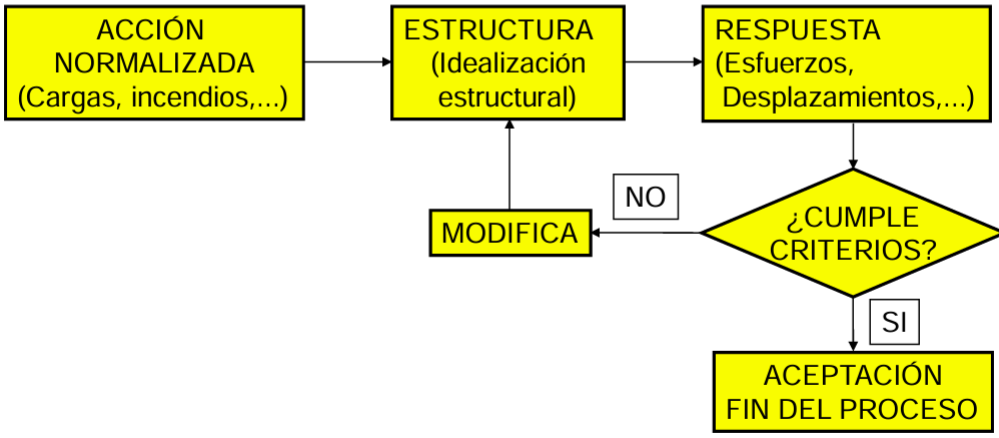
\includegraphics[width=0.75\linewidth]{Imagenes/Proyecto estructural. Procedimiento (1).png}

\end{figure}

\subsection{Objetivos en estructuras nuevas.}
Crear estructuras que cumplan los siguientes requisitos o criterios:
\begin{itemize}
    \item Resistencia: Las estructuras deben de resistir las solicitaciones a las que pueden estar expuestas durante su vida útil.
    \item Rigidez: Las estructuras deben de tener rigidez adecuada para impedir que se produzcan movimientos que afecten a su uso o a componentes no estructurales vinculados a ella.
    \item Estabilidad: Que la estructura no se desmorone por inestabilidad total o parcial.
    \item Durabilidad: Que la capacidad resistente no varía ostensiblemente a lo largo del tiempo.
    \item Ductilidad: Que se puedan evitar los fallos frágiles ``sin previo aviso''.
\end{itemize}

\subsection{Objetivos en estructuras existentes.}
Se han de seguir las siguientes etapas:
\begin{enumerate}
    \item Auscultación del estado real de la estructura.
    \begin{itemize}
        \item Ensayo in-situ.
        \item Modelos numéricos actualizados a partir de los ensayos.
    \end{itemize}
    \item Diseño del reacondicionamiento.
    \begin{itemize}
        \item Establecer prioridades de actuación.
        \item Cribado previo de detalles.
        \item Tanteos simples.
        \item Métodos detallados.
    \end{itemize}
    \item Proyecto final de esfuerzo o demolición.
\end{enumerate}

\section{Aspectos generales de un proyecto estructural. Fases (anteproyecto, básico y ejecución). Normas.}
Fases de un proyecto estructural:
\begin{itemize}
    \item Anteproyecto: Expone los aspectos fundamentales y las características generales de la intervención.
    \item Proyecto Básico: Define de modo preciso las características generales de la intervención mediante la adopción de soluciones concretas y su justificación.
    \item Proyecto de Ejecución: Desarrolla el Proyecto Básico con determinación completa de detalles y especificaciones de todos los materiales, elementos, sistemas constructivos y equipos.
\end{itemize}

Las normas proporcionan las bases de cálculo así como los criterios a comprobar para garantizar la seguridad de la estructura proyectada.

Las bases de cálculo deben de proporcionar, entre otros aspectos, la siguiente información:
\begin{itemize}
    \item Acciones: Cualquier causa (fuerza o deformación) capaz de producir o modificar estados tensiónales en una estructura. Las acciones pueden ser permanentes, variables en el tiempo o accidentales. Además pueden ser libres o fijas en el espacio.
    \item Situación: Condiciones en la que se puede encontrar una estructura a lo largo de su vida útil.
    \item Combinación de acciones: Para evaluar las solicitaciones sobre una estructura, las distintas posibles acciones se combinan entre sí con el objeto de representar situaciones determinadas, ponderando su valor dependiendo de su importancia.
\end{itemize}

\section{Elementos estructurales y no estructurales. Elementos estructurales primarios y secundarios.}
Elementos estructurales: Son los elementos que soportan los esfuerzos y deformaciones que tiene una determinada estructura. Son parte de la estructura (vigas, pilares, losas, muros, zapatas...).

\begin{figure}[h]
    \centering
    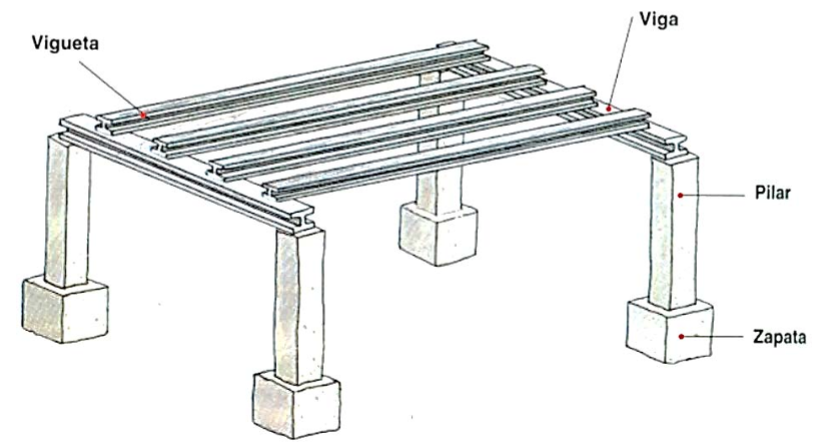
\includegraphics[width=0.75\linewidth]{Imagenes/Elementos estructurales.png}
    \caption{Elementos estructurales.}
\end{figure}

Elementos no estructurales: Componentes de un edificio que están unidos a las partes estructurales (componentes arquitectónicos: tabiques, ventanas, puertas,...) que cumplen funciones esenciales en el edificio (componentes mecánicos y eléctricos: calefacción, instalaciones eléctricas,...) o que están simplemente dentro de las edificaciones (muebles,...)

Elementos estructurales primarios: Constituyen la vía para transmitir las cargas horizontales y verticales que actúan sobre el edificio al terreo (pórticos principales, sus uniones y sus cimentaciones).

Elementos estructurales secundarios: Son los elementos estructurales que transmiten las cargas a los elementos principales (vigas secundarias o correas).

\begin{figure}[h]
    \centering
    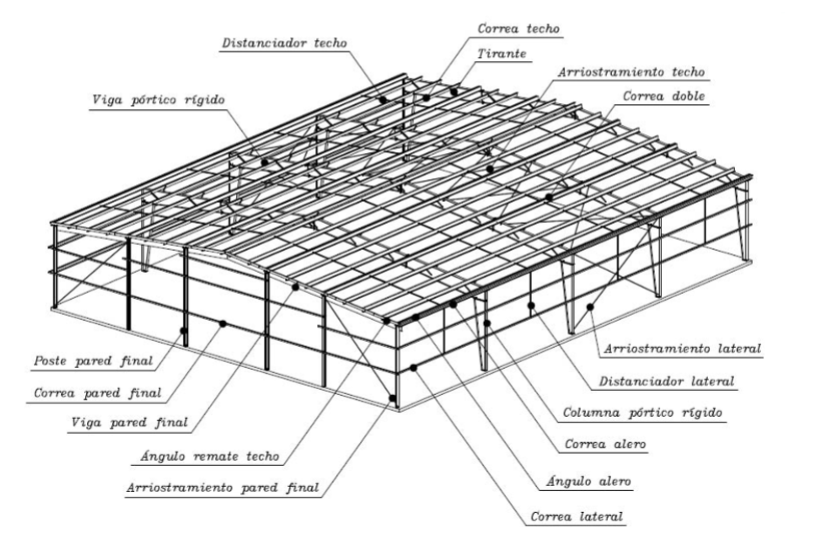
\includegraphics[width=0.75\linewidth]{Imagenes/Elementos estructurales (1).png}
    \caption{Elementos estructurales primarios y secundarios.}
\end{figure}

\section{Seguridad: Métodos en tensiones admisibles y métodos en estado límite. ELU y ELS.}
Para garantizar la seguridad de una estructura existen diversos métodos en función de cómo se aborde el problema.

\subsection{Método en tensiones admisibles (base determinista).}
En el método en tensiones admisibles se calcula la tensión $\sigma$ en la sección más solicitada y, después, para el material en cuestión, cuya resistencia máxima útil es $\sigma_{mat}$, se escoge un esfuerzo máximo admisible $\sigma_{adm}$. Para garantizar la seguridad se ha de verificar:

\begin{equation}
    \sigma \leq \sigma_{adm} = \frac{\sigma_{mat}}{FS}
\end{equation}

siendo $FS$ un factor de seguridad cuyo objetivo es disminuir la posibilidad de fallo en la estructura.

\subsubsection{Consecuencias.}
\begin{itemize}
    \item Mayor desaprovechamiento de la capacidad resistente de los materiales, ya que no se considera su capacidad de readaptación plástica.
    \item No nos da ninguna información sobre el margen de seguridad de la estructura, es decir, cuánta más carga puede recibir hasta su rotura.
    \item De lo anterior se deduce que, con este método, se construirán estructuras más caras e inciertas en cuanto a seguridad.
\end{itemize}

\subsection{Bases probabilista para el proyecto estructural.}

\begin{figure}[h]
    \centering
    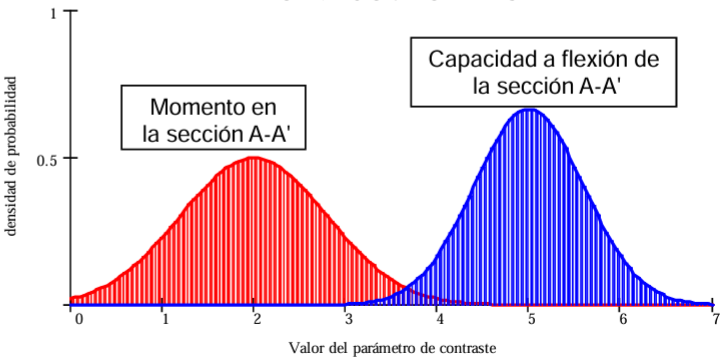
\includegraphics[width=0.75\linewidth]{Imagenes/Aproximacion probabilistica.png}
    \caption{Aproximación probabilística.}
\end{figure}

Al proyectar una estructura existen efectos aleatorios que provocan incertidumbre en aspectos tales como las propiedades del material, las incertidumbres en la carga, el proceso de idealización estructural y de cálculo, las características geométricas reales y la estructura y la variación en el tiempo de las propiedades mecánicas de la estructura y las acciones sobre la misma. En el enfoque probabilista, toda esta variabilidad se estima con base estadística utilizando las funciones de densidad de probabilidad.

Nivel 2: La variables de carga y resistencia se representan por sus funciones estadísticas de distribución.

Nivel 1: Se obtienen realizando simplificaciones sobre los métodos del nivel 2.
\begin{itemize}
    \item Engloba los efectos de las diferentes causas de incertidumbre en dos factores: Resistencia de los materiales (R) y valores de las acciones (S).
    \item Sustituye las funciones de distribución de estos dos parámetros por su valores característicos.
    \item Pondera estos valores utilizando unos coeficientes parciales de seguridad que tienen en cuenta los factores aleatorios.
    \item Los coeficientes parciales de seguridad se definen para una fiabilidad dada.
    \item La EHE y casi todos los códigos técnicos (CTE, EC2, ACI,...) se basan en el nivel 1 de diseño.
\end{itemize}

\begin{figure}[h]
    \centering
    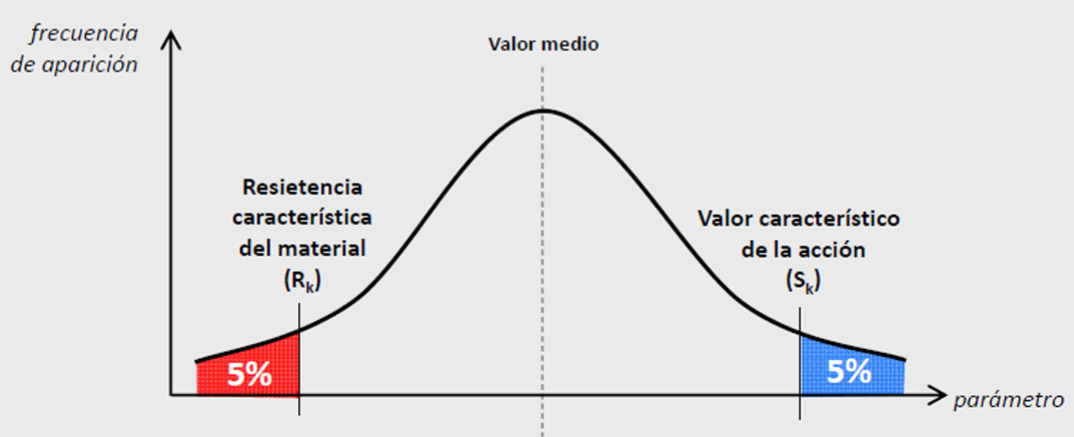
\includegraphics[width=0.75\linewidth]{Imagenes/Valor caracteristico resistencia accion.png}
    \caption{Probabilidad de aparición.}
\end{figure}

Valor característico de la resistencia: Valor para el cual existe una probabilidad del $5\%$ de que existan valores más bajos de resistencia.

Valor característico de la acción: Valor para el cual existe una probabilidad del $5\%$ de que existan valores más altos de la acción.

\subsection{Coeficientes parciales de seguridad.}
\begin{itemize}
    \item Tienen en cuenta las incertidumbres que introducen en el cálculo los factores aleatorios del proyecto.
    \item Se definen un coeficiente parcial de minoración de resistencias, $\gamma_m$, y un coeficiente parcial de mayoración de acciones, $\gamma_f$, de tal forma que el riesgo de fallo estructural sea tolerable.
    \item Aplicando los coeficientes parciales de seguridad se obtienen los valores de cálculo.
    \item La determinación de los coeficientes parciales de seguridad debe ser un compromiso entre el coste de construcción y conservación de la estructura (aumenta con el coeficiente de seguridad) y el coste de los daños potenciales para el riesgo asumido (disminuye al aumentar el coeficiente de seguridad).
\end{itemize}

\subsection{Estados límites.}
Constituyen la expresión precisa d los conceptos generales de fallo y se formulan en la práctica como simple relación de formas de fallo que han de comprobarse, es decir, se establecen límites o situaciones que, al rebasarse, hacen que la estructura no cumpla algunas de las funciones para las que fue proyectada.

Por ejemplo: en vez de decir que un tornillo no se puede romper, precisar las formas de fallo que se han de comprobar: rotura de la caña yo del núcleo a corte o tracción, pérdida de la rosca, aplastamiento contra la chapa.

\subsubsection{Clasificación.}
Se postulan situaciones relativas a:
\begin{itemize}
    \item la funcionalidad (E. L. de Servicio)
    \begin{itemize}
        \item Se relacionan con la funcionalidad, estética y durabilidad de la estructura.
        \item Se utilizan las combinaciones de carga con alta probabilidad de ocurrencia.
        \item Los parámetros de control son desplazamientos, aceleraciones.
    \end{itemize}
    \item la seguridad (E. L. Último)
    \begin{itemize}
        \item Se utilizan las combinaciones de carga con baja probabilidad de ocurrencia-
        \item Se relacionan con la seguridad que ofrece la estructura frente al colapso total o parcial.
        \item Los parámetros de control son los esfuerzos.
    \end{itemize}
\end{itemize}

\begin{figure}[h]
    \centering
    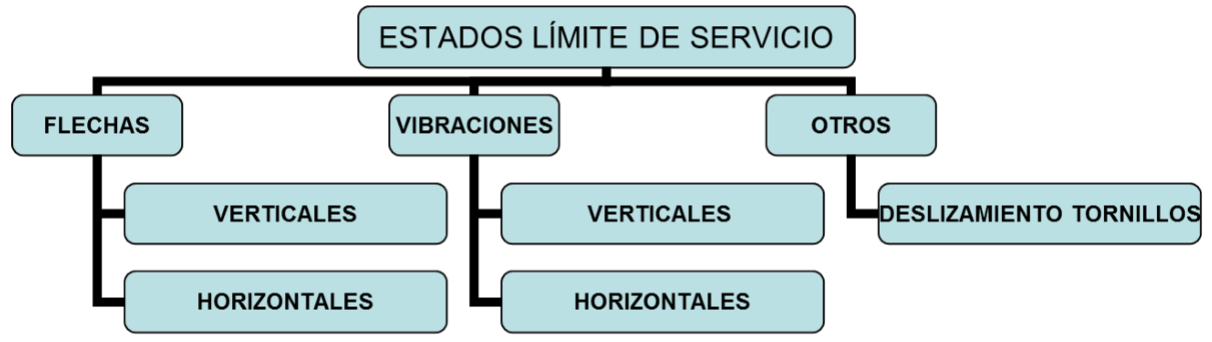
\includegraphics[width=\linewidth]{Imagenes/Estados limite de servicio.png}
\end{figure}

\begin{equation}
    C_d \geq E_d
\end{equation}
Valor límite admisible para el Estado Límite a comprobar $\geq$ Valor de cálculo obtenido por el efecto de la acción.

\begin{figure}[h]
    \centering
    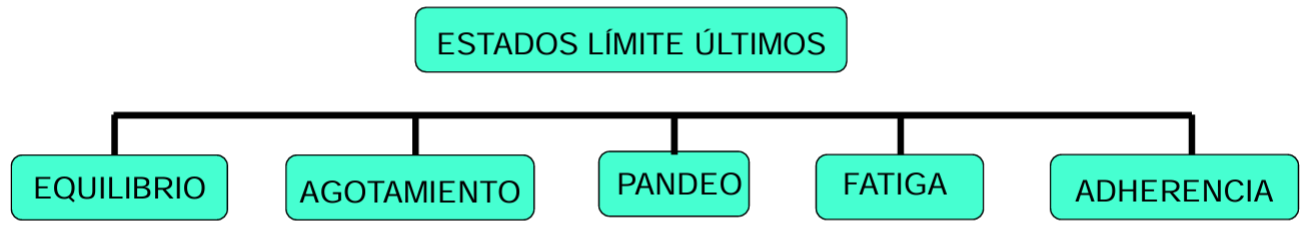
\includegraphics[width=\linewidth]{Imagenes/Estados limite ultimos.png}
\end{figure}

\begin{equation}
    R_d \geq S_d
\end{equation}
Capacidad de respuesta de la estructura $\geq$ Valor de cálculo obtenido por el efecto de la acción.